\documentclass[conference]{IEEEtran}
\usepackage{graphicx}
\usepackage{tikz}
 
\usepackage[colorlinks = true, citecolor = blue]{hyperref}

% math lib
\usepackage{amsmath}
\usepackage{mathrsfs}

% operators
\DeclareMathOperator*{\argmax}{arg\,max}
\DeclareMathOperator*{\argmin}{arg\,min}
\newcommand\ceiling[1]{\left\lceil #1 \right\rceil}

% empty set
\usepackage{amssymb}
\let\emptyset=\varnothing

% algorithms
\usepackage{algorithm}
\usepackage{algorithmic}
\renewcommand{\algorithmicrequire}{\textbf{Input:}}
\renewcommand{\algorithmicensure}{\textbf{Output:}}

\begin{document}
% --------------------------------------------
% --------------Change HERE! -----------------
% --------------------------------------------
\def\authorone{Han Qiu}
\def\groupid{2}
% --------------------------------------------
\title{CS258 Final Report: The RSA Problem}
\author{
    \IEEEauthorblockN{\authorone}
    \IEEEauthorblockA{
        Group \groupid
    }    
}

\maketitle
\IEEEpeerreviewmaketitle


\section{Methods: RL-based Routing}
\subsection{RL Algorithms}
Reinforcement learning (RL) algorithms enable agents to learn optimal policies through interactions with an environment, aiming to maximize accumulated rewards. Among these, Proximal Policy Optimization (PPO) stands out due to its efficiency and stability. PPO, introduced by Schulman et al. \cite{schulman2017proximal}, is a policy gradient method that optimizes a "surrogate" objective function. This function limits the update at each step, helping to avoid large, destructive policy updates and ensuring more stable learning.

PPO achieves this stability by using a clipped probability ratio between the old and new policies, thus ensuring that the updates remain within a small range around 1. This clipping mechanism prevents the policy from changing too drastically, which is a common issue in other policy optimization methods. The core advantage of PPO is its simplicity and its ability to perform well across a wide range of environments with minimal hyperparameter tuning.

% Example algorithm box
\begin{algorithm}[H]
\caption{Proximal Policy Optimization}
\begin{algorithmic}
\REQUIRE Initial policy parameters $\theta_0$, initial value function parameters $\phi_0$
\ENSURE Optimized policy parameters $\theta^*$
\FOR{iteration $= 1, 2, \dots$}
    \STATE Collect set of trajectories $\mathcal{D}_k$ by running policy $\pi_{\theta_{k-1}}$ in the environment.
    \STATE Compute rewards-to-go $\hat{R}_t$.
    \STATE Compute advantage estimates $\hat{A}_t$ using the current value function $V_{\phi_{k-1}}$.
    \STATE Optimize surrogate objective:
    \begin{equation}
    \begin{aligned}
        & \argmax_{\theta} \frac{1}{|\mathcal{D}_k| T} \sum_{\tau \in \mathcal{D}_k} \sum_{t=0}^T \min \left( \frac{\pi_\theta(a_t | s_t)}{\pi_{\theta_{k-1}}(a_t | s_t)} \hat{A}_t, \right. \\
        & \quad \left. \text{clip}\left(\frac{\pi_\theta(a_t | s_t)}{\pi_{\theta_{k-1}}(a_t | s_t)}, 1-\epsilon, 1+\epsilon\right) \hat{A}_t \right)
    \end{aligned}
    \end{equation}
    \STATE Update policy parameters $\theta_k = \theta$.
    \STATE Optionally update the value function parameters $\phi_k$ by regression on $\hat{R}_t$.
\ENDFOR
\end{algorithmic}
\end{algorithm}

\textit{Note:} PPO is particularly useful in scenarios where the interaction with the environment is expensive or the policy evaluation is noisy, making it a robust choice for many practical applications, including robotics and game playing.

\subsection{State Space}
The state space for the reinforcement learning environment in Case I is defined as follows:
\begin{verbatim}
self.observation_space = spaces.Box(
    low=0, high=1, shape=(7,), dtype=np.float32)
\end{verbatim}
In this definition, the observation space is a 7-dimensional vector where each component can take a value between 0 and 1. Which represents the utilization of 7 edges in "San Diego Supercomputer Center to Jon Von Neumann Center, Princeton, NJ"

\subsection{Action Space}
The action space in my reinforcement learning model is defined as a discrete space with two possible actions. 
\begin{verbatim}
self.action_space = spaces.Discrete(2)
\end{verbatim}
which represents two different routing paths from San Diego Supercomputer Center to Jon Von Neumann Center, Princeton, NJ.
\subsection{Reward Function}
The reward function in my reinforcement learning environment plays a critical role in shaping the agent's behavior by providing feedback on the effectiveness of the actions taken. It is designed to encourage certain outcomes while discouraging others. The reward mechanism is implemented as follows:
\begin{verbatim}
if color is not None:
    reward = 2   
else:
    reward = -1
\end{verbatim}
In this implementation, a reward of 2 is given when a `color` is successfully assigned to a routing path, indicating a successful allocation of resources. Conversely, a reward of -1 is issued when no `color` can be assigned, signifying a failed routing attempt. This setup aims to motivate the agent to find solutions that maximize resource utilization efficiently, thereby improving the overall performance of the network routing strategy.

\section{Method: Spectrum Allocation}
For spectrum allocation, I use the same index-based allocation algorithm in Assignment 4. which is greedy color selection (smaller index first)
% Explain your heuristic
% If you have multiple, you can make subsections 

% If you borrow some ideas from papers, cite them with bibtex (e.g. \cite{8509143})


\section{Results}
\subsection{Learning Curve}
The learning curve is an essential indicator of the performance and efficiency of the reinforcement learning model over time. It demonstrates how the agent improves its ability to make decisions as it gains experience through episodes. 

\begin{figure}[htbp]
\centering
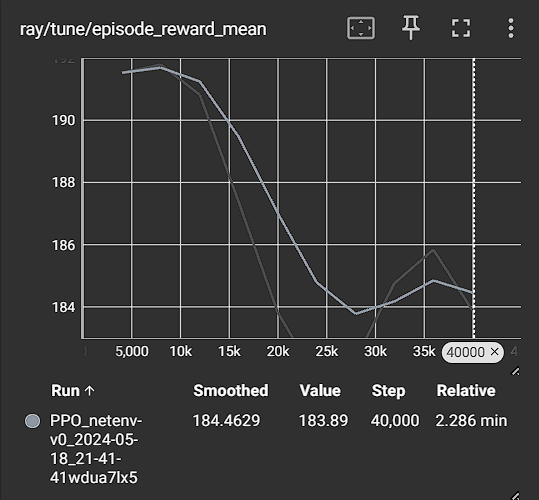
\includegraphics[width=0.48\textwidth]{rewardvsepisode.png}
\caption{Learning curve showing how rewards change as the number of episodes increases.}
\label{fig:learningcurve}
\end{figure}
The graph looks weird, this might be because the implementation errors in my environment. I am expecting an ascending graph to show that the agent is learning.  
% Insert figures
% Explain the results

\subsection{Utilization (The Objective)}
The primary objective is to maximize the utilization of optical resources across the network. Let \( c(e) \) denote the capacity of a link \( e \). The occupied slots at time \( t \) on link \( e \) are represented as \( o_t(e) \). Consequently, the utilization \( u_t(e) \) of link \( e \) at time \( t \) can be computed by the equation:
\begin{equation}
u_t(e) = \frac{o_t(e)}{c(e)}
\end{equation}

Furthermore, the average utilization \( U(e) \) of a link \( e \) over \( T \) episodes (equivalent to \( T \) arrivals of requests) is defined as:
\begin{equation}
U(e) := \frac{1}{T} \sum_{t=0}^{T-1} \frac{o_t(e)}{c(e)}
\end{equation}

The formal objective of achieving maximum network-wide utilization is defined as follows. Let \( E \) denote the set of all links in the network. We define the network-wide utilization \( U_1 \) as the average of the total utility of all edges:
\begin{equation}
\text{maximize } U := \frac{1}{|E|} \sum_{e \in E} U(e)
\end{equation}

\begin{figure}[htbp]
\centering
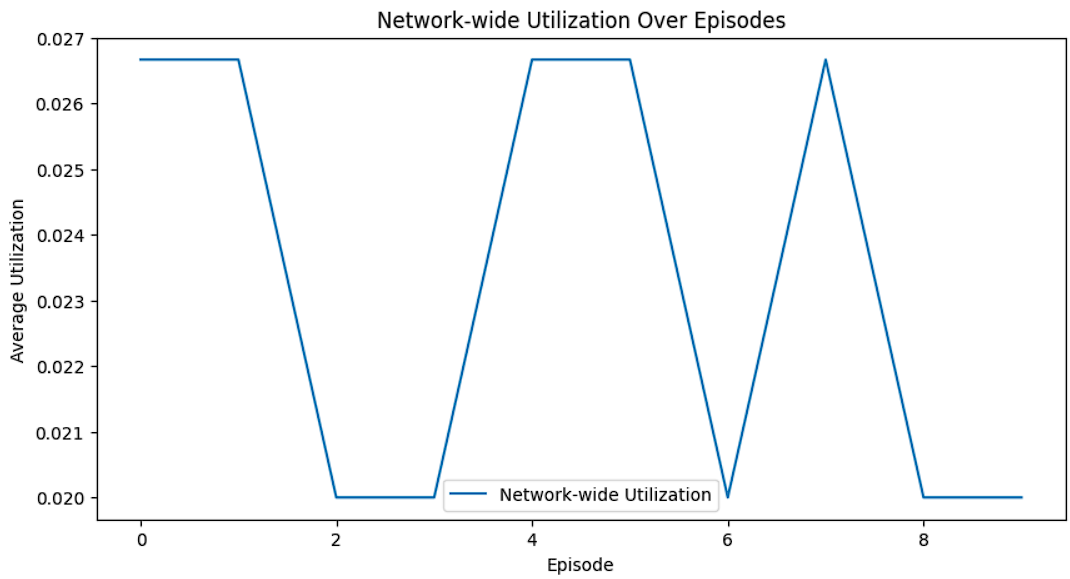
\includegraphics[width=0.48\textwidth]{objvsepisode.png}
\caption{this graph showing how the network-wide utilization changes as the number of episodes increases.}
\label{fig:objective}
\end{figure}
The configuration need to be adjust to get better utilization graph.

\subsection{Comparison}
\begin{figure}[htbp]
\centering
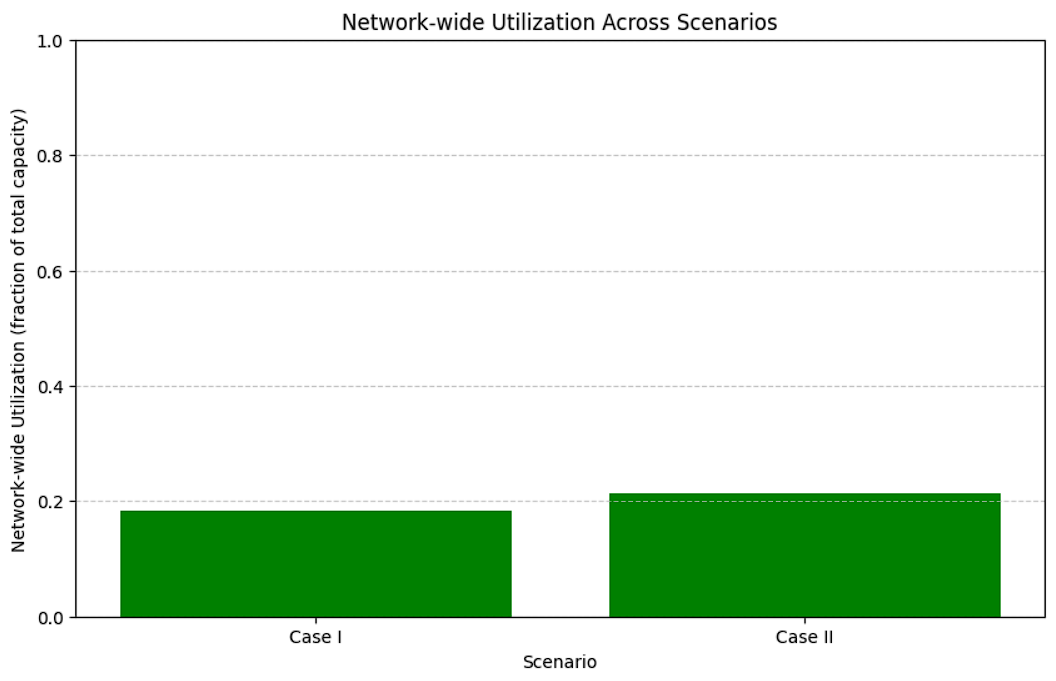
\includegraphics[width=0.48\textwidth]{noRL.png}
\caption{the values of the objective obtained by simple heuristics.}
\label{fig:objectivevalue}
\end{figure}
the values of the objective obtained by simple heuristics: 0.18 for case I, 0.21 for case II. Reinforcement Learning with PPO for case I is 0.26. The result of Reinforcement Learning is not ideal, need future improvement.

\section{Conclusion and Future Work}
The RSA problem with Reinforcement Learning PPO performs better than simple heuristics, but my result is not ideal.
Future improvement is expected, including implementation and configuration.

\bibliography{ref}
\bibliographystyle{ieeetr}


\end{document}



